\chapter{Protein Modelling}
\label{chapter:protein_modelling}

\begin{quote}
``Certainly no subject or field is making more progress on so many fronts at the present moment, than biology, and if we were to name the most powerful assumption of all, which leads one on and on in an attempt to understand life; it is that all things are made of atoms, and that everything that living things do can be understood in terms of jigglings and wigglings of atoms.'' \\
--- \textit{Richard Feynman, Nobel Prize Winner 1965}
\end{quote}

\section{Protein Modelling and Simulation}

This chapter discusses the important aspects of protein modelling and simulation, including the most popular methods and algorithms.
The chapter concludes with a more detailed discussion of the specific method classes which relate to the work described in this thesis.
\subsection{The Sequence-to-Structure deficit}

The rapid explosion in the number of available protein sequences is largely due to the success of  numerous genome-sequencing projects which are currently underway. The recently completed human  and other model organism genome sequencing projects alone have produced in excess of 250,000 expressed gene sequences in over 1,000 genomes. By contrast to this, an overview in 2004 stated that the PDB contained only $\sim$23,000 structures\cite{NATIVE:PDB:B}.
In the coming years, it is the task of structural biologists and bioinformaticians to fill the void between the known genome and the known structural proteome.


The primary experimental methods that are currently used to produce atomic resolution structures are \xray\ Crystallography and Nuclear Magnetic Resonance (NMR). Both these methods however are highly human-time intensive and require that the protein of interest can be expressed in sufficient quantities and purified to a high concentration. Other specific sub-groups of proteins, particularity membrane proteins, have additional properties that make experimental structure resolution inherently difficult. Therefore, to be able to experimentally resolve the structure of every protein of biological interest is scarcely feasible; \insilico\ modelling provides a highly attractive alternative with the caveat that, to be of genuine use, the models
produced \emph{must} describe protein structure to atomic resolution with a high degree of confidence.


\subsection{Structure Prediction}

Structure prediction is theoretically possible as it has been shown that the tertiary structure of a protein is dictated by its primary sequence alone\cite{NATIVE:Anfinsen1973}.
Predicting the tertiary structure from primary sequence was first attempted by Nemethy and Scheraga in 1965\cite{COMPCHEM:Nem65} and has since been an active area of research. Current techniques for protein structure prediction fall into three main groups -- comparative modelling, fold recognition, and \abinitio\ methods -- in decreasing order of reliance on known structure and increasing difficulty.

All protein structure prediction methods comprise three fundamental attributes. Firstly, a protein representation
is chosen which is required to be the  lowest complexity capable of reproducing the desired protein-like features. Secondly, some form of scoring function,
usually termed a ``forcefield'', is required to attempt the calculation of a good approximation to the real free energy of the system. This scoring function can be defined using a large number of approaches, ranging from knowledge-based statistically-derived functions to entirely physico-chemical functions. Finally, a conformational search method is required, which attempts to provide good coverage of conformational space, with the ultimate aim of locating the global energy minimum. The search itself is not a trivial problem as protein conformational space is both highly multi-dimensional and contains an extraordinary large number of competing local energy minima. The specific
details of choosing a protein representation, forcefield and conformational
search method are discussed further in sections \ref{section:protein_rep}, \ref{section:protmodel:energy_functions}
and \ref{section:protmodel:conformational_search} respectively.
These three elements can be developed, calibrated and evaluated separately, but are intertwined in the modelling process itself -- The search process
must be compatible with the chosen protein representation and will be directed by the results of the chosen energy functions.
 
Due to the limited nature of computational resources, \insilico\   methods must be developed which minimise the conformational space which must be explored, as well as using forcefields
which adequately define the  free energy of a given conformation. This represents the hugely complex task of protein structure prediction. Once \insilico\ prediction has truly matured it will no doubt be the method of choice for solving
the structure of all but the most unusual proteins. For the time being, however, all these methods come with associated difficulties. 


\subsection{CASP}
\label{section:prot_model:casp}

\casp, which stands for Critical Assessment of Techniques for Protein Structure Prediction, is a community-wide competition which has taken place every two years since 1994\cite{METHOD:CASP6}.
Its twofold aim is to provide a critical review of the current state of the
field and to allow research groups to perform genuine blind
tests on their respective prediction methodologies. During this work, predictions were submitted to \casp-7 and are presented in chapter \ref{chapter:casp}.

Briefly, the organisers of \casp\ release amino acid sequences  of proteins for which an experimental
structure is about to be published. The modelling community is then allowed
around two weeks to generate and select their models for each given
target sequence. The results are quantitatively analysed by the organisers and subsequently
conclusions are drawn.

Since \casp-7, method category nomenclature was redefined to reflect developments in current methods. The ``Template-based modelling'' category now includes all traditional comparative modelling, homologous fold based models and some easier analogous-fold-based models. As in \casp-6, the ``Template-free modelling'' category  includes models of proteins with previously unseen folds and difficult analogous-fold-based models.
These methodologies are described further below.



\subsection{Template-free Modelling}

Template-free methods attempt to predict protein structures using their primary
sequence as the only direct source of information; by definition they do not use whole protein templates\cite{METHOD:CASP6:NEWFOLD}.
Current template-free methodologies handle \al-helical-only proteins far more effectively than those containing \be-strands, mainly due to the difficulties
of dealing with strand register and high contact-order topologies\cite{NATIVE:Lackner1999}. Indeed, all structure involving contacts which are far apart in sequence
space are more difficult
to predict; mainly because the organisation of such contacts proves harder for conformational change
algorithms. At the time of writing, \abinitio\ methods cannot compete with the more empirical methods of structure prediction.

A subset of methods within this class, termed pure \abinitio\ methods, use
only the protein sequence and fundamental physical laws in order to predict the structure
of a protein, although these are comparatively computationally expensive and
so only applicable to smaller proteins\cite{COMPCHEM:Gib2001}. Some other more rapid methods, which arguably misuse the term \abinitio, are 
trained on libraries of known structures\cite{NATIVE:Sippl1992}, or involve energy functions derived from structural database information\cite{NATIVE:Sippl1996}.

The most successful modelling class is the fragment assembly methods, which are
sometimes referred to as \denovo\ methods. Such methods
stitch together and refine short fragments derived from the PDB\cite{METHOD:Rosetta}. Success is attributed to the fact that use of these fragments
implicitly accounts for  local structural propensities of each individual sequence.










\subsection{Template-based Modelling}

Template-based modelling methodologies all rely heavily on one or more
structural templates and usually on statistical information directly
derived from the PDB. There are two main approaches used in this class of methods. The first is
comparative modelling, which aims to predict a proteins structure using a
template of high sequence identity to the protein of interest. The
second is threading-based methods which score the energetic stability
of a given sequence within multiple possible protein folds. 

\subsubsection{The Strength of Template Modelling}



The underlying principle which makes template-based modelling so appealing is
that it seems certain that the great majority (\textgreater95\%) of the protein sequence families belong to just $\sim$1,000 common folds\cite{SEQUENCE:Zuck75}.
Other more recent estimates, that have used very different criteria, produce similar estimates of between
700 and 4,000 independent folds\cite{NATIVE:Govindarajan1999,NATIVE:Wolf2000,NATIVE:Zhang1998}; tiny numbers in comparison to the number of
different protein structures in nature. 

One such fold, the immunoglobulin\cite{BIOLOGY:Wil88} (Ig) super-fold, is a frequent motif of interest to many molecular biologists. Indeed many large immunoglobulin-like sequence families are to be found in the various  representative sequence databases. The Ig fold exemplifies that, following gene duplication and subsequent sequence divergence, a stable fold can be modified to provide thousands of novel functional roles. 

The sequence$\to$structure relationships for
three such Ig domains are illustrated in figure \ref{fig:intro:seqstrucrelationship}.
For all natural proteins discovered so far, moderate sequence-identity implies
a high degree of  structural similarity as evolution conserves protein structure over sequence\cite{NATIVE:Chothia1986}. 
In this figure, 2GK2A is first compared to 2DKSA and then to 1L6ZA, which share
72\% and 42\% sequence identity respectively. Following superimposition, a number of   structural traits are clear. 

The first is that even at just 42\% sequence identity, the level
of structural conservation is profound. It is known that structures with as little as 20\% sequence identity can still yield structures which still adopt the same overall topology\cite{NATIVE:SUPERFAMILY:2007}.
It is common for the hydrophobic core to
remain largely constant in terms of  both residue identity and packing within surprisingly high levels of sequence divergence \cite{STRUCTURE:Rod98}.
Indeed, in  figure \ref{fig:intro:seqstrucrelationship}
the core of the protein is clearly
almost completely identical, and where residues are different, they are almost
exclusively exchanged for alternatives with similar basic chemical properties.

 
Secondly, where there is sequence divergence, it is almost entirely in surface regions with corresponding structural divergence. These  surface structural modifications
are often extremely important to the
introduction of new function.
Such structurally variable
regions must be built during any modelling process, in the absence of structural template information.

 

\begin{figure}[p]

\begin{center}

\mbox{
      \subfigure[Structural alignment of 2GK2A to 2DKSA.]%
      {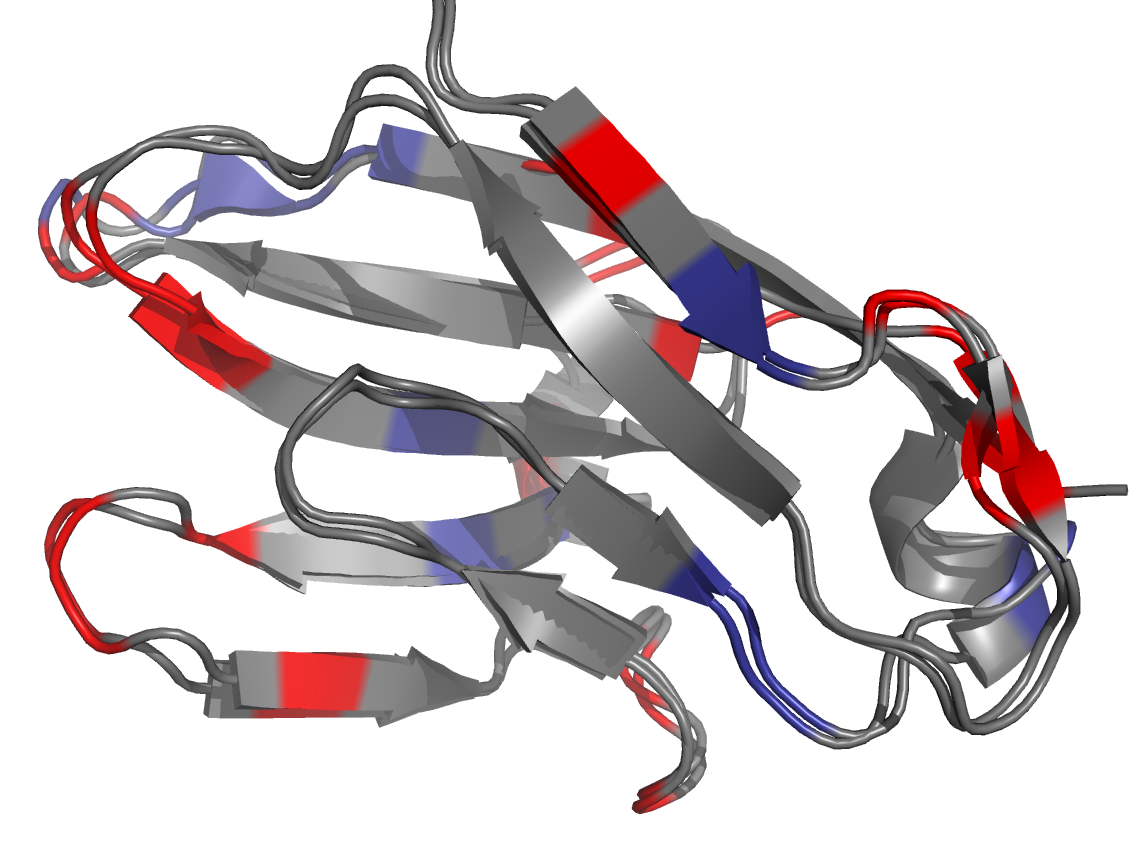
\includegraphics[width=0.58\textwidth]{02-ProtModelling/comparative/comp_72.png}}
}
 
 \mbox{
      \subfigure[High identity alignment: Alignment of 2GK2A length 111 and 2DKSA length 130. Alignment yields 80/111 (72\%)  identities and 92/111 (83\%) positives.]{
      
\begin{minipage}{0.9\textwidth}
\begin{tiny}
\tt %makes the font fixed-width so that all the columns line-up
\begin{tabbing}

\ \ \ \ \ \ \=1\ \ \ \ \ \ \ \ 10\ \ \ \ \ \ \ \ 20\ \ \ \ \ \ \ \ 30\ \ \ \ \ \ \ \ 40\ \ \ \ \ \ \ \ 50\ \ \ \ \ \ \ \ 60\ \ \ \ \ \ \ \ 70\ \ \ \ \ \ \ \ 80\ \ \ \ \ \ \ \ 90\ \ \ \ \ \ \ \ 100\ \ \ \ \ \ \ \ 111 \\
\>|\ \ \ .\ \ \ \ |\ \ \ \ .\ \ \ \ |\ \ \ \ .\ \ \ \ |\ \ \ \ .\ \ \ \ |\ \ \ \ .\ \ \ \ |\ \ \ \ .\ \ \ \ |\ \ \ \ .\ \ \ \ |\ \ \ \ .\ \ \ \ |\ \ \ \ .\ \ \ \ |\ \ \ \ .\ \ \ \ |\ \ \ \ .\ \ \ \ .| \\
2GK2A\ \textcolor{black}{SG}\textcolor{Red}{G}\textcolor{black}{AQLT}\textcolor{Red}{T}\textcolor{black}{E}\textcolor{RoyalBlue}{SM}\textcolor{black}{P}\textcolor{Red}{F}\textcolor{black}{N}\textcolor{Red}{V}\textcolor{black}{AEGKEVLLLVHNLPQ}\textcolor{Red}{QLF}\textcolor{black}{GY}\textcolor{RoyalBlue}{S}\textcolor{black}{WYKGE}\textcolor{Red}{R}\textcolor{black}{VD}\textcolor{Red}{G}\textcolor{black}{NR}\textcolor{RoyalBlue}{Q}\textcolor{black}{I}\textcolor{RoyalBlue}{V}\textcolor{black}{GY}\textcolor{Red}{A}\textcolor{black}{I}\textcolor{Red}{GT}\textcolor{black}{QQ}\textcolor{Red}{A}\textcolor{black}{TPGPA}\textcolor{Red}{N}\textcolor{black}{S}\textcolor{Red}{G}\textcolor{black}{RETIYPNASLL}\textcolor{RoyalBlue}{IQ}\textcolor{black}{NVT}\textcolor{RoyalBlue}{Q}\textcolor{black}{NDTG}\textcolor{Red}{F}\textcolor{black}{YTLQVIK}\textcolor{Red}{S}\textcolor{RoyalBlue}{D}\textcolor{black}{L}\textcolor{RoyalBlue}{VN}\textcolor{black}{EE}\textcolor{Red}{A}\textcolor{black}{TGQF}\textcolor{Red}{H}\textcolor{black}{VY}
\\
\>\textcolor{black}{SG}\textcolor{Red}{\ }\textcolor{black}{AQLT}\textcolor{Red}{\ }\textcolor{black}{E}\textcolor{RoyalBlue}{++}\textcolor{black}{P}\textcolor{Red}{\ }\textcolor{black}{N}\textcolor{Red}{\ }\textcolor{black}{AEGKEVLLLVHNLPQ}\textcolor{Red}{\ \ \ }\textcolor{black}{GY}\textcolor{RoyalBlue}{+}\textcolor{black}{WYKGE}\textcolor{Red}{\ }\textcolor{black}{VD}\textcolor{Red}{\ }\textcolor{black}{NR}\textcolor{RoyalBlue}{+}\textcolor{black}{I}\textcolor{RoyalBlue}{+}\textcolor{black}{GY}\textcolor{Red}{\ }\textcolor{black}{I}\textcolor{Red}{\ \ }\textcolor{black}{QQ}\textcolor{Red}{\ }\textcolor{black}{TPGPA}\textcolor{Red}{\ }\textcolor{black}{S}\textcolor{Red}{\ }\textcolor{black}{RETIYPNASLL}\textcolor{RoyalBlue}{++}\textcolor{black}{NVT}\textcolor{RoyalBlue}{+}\textcolor{black}{NDTG}\textcolor{Red}{\ }\textcolor{black}{YTLQVIK}\textcolor{Red}{\ }\textcolor{RoyalBlue}{+}\textcolor{black}{L}\textcolor{RoyalBlue}{++}\textcolor{black}{EE}\textcolor{Red}{\ }\textcolor{black}{TGQF}\textcolor{Red}{\ }\textcolor{black}{V+} \\
2DKSA\ \textcolor{black}{SG}\textcolor{Red}{T}\textcolor{black}{AQLT}\textcolor{Red}{I}\textcolor{black}{E}\textcolor{RoyalBlue}{AV}\textcolor{black}{P}\textcolor{Red}{S}\textcolor{black}{N}\textcolor{Red}{A}\textcolor{black}{AEGKEVLLLVHNLPQ}\textcolor{Red}{DPR}\textcolor{black}{GY}\textcolor{RoyalBlue}{N}\textcolor{black}{WYKGE}\textcolor{Red}{T}\textcolor{black}{VD}\textcolor{Red}{A}\textcolor{black}{NR}\textcolor{RoyalBlue}{R}\textcolor{black}{I}\textcolor{RoyalBlue}{I}\textcolor{black}{GY}\textcolor{Red}{V}\textcolor{black}{I}\textcolor{Red}{SN}\textcolor{black}{QQ}\textcolor{Red}{I}\textcolor{black}{TPGPA}\textcolor{Red}{Y}\textcolor{black}{S}\textcolor{Red}{N}\textcolor{black}{RETIYPNASLL}\textcolor{RoyalBlue}{MR}\textcolor{black}{NVT}\textcolor{RoyalBlue}{R}\textcolor{black}{NDTG}\textcolor{Red}{S}\textcolor{black}{YTLQVIK}\textcolor{Red}{L}\textcolor{RoyalBlue}{N}\textcolor{black}{L}\textcolor{RoyalBlue}{MS}\textcolor{black}{EE}\textcolor{Red}{V}\textcolor{black}{TGQF}\textcolor{Red}{S}\textcolor{black}{VH}
\\
\>|\ \ \ |\ \ \ \ .\ \ \ \ |\ \ \ \ .\ \ \ \ |\ \ \ \ .\ \ \ \ |\ \ \ \ .\ \ \ \ |\ \ \ \ .\ \ \ \ |\ \ \ \ .\ \ \ \ |\ \ \ \ .\ \ \ \ |\ \ \ \ .\ \ \ \ |\ \ \ \ .\ \ \ \ |\ \ \ \ .\ \ \ \ |\ \ \ \ .| \\
\>6\ \ \ 10\ \ \ \ \ \ \ \ 20\ \ \ \ \ \ \ \ 30\ \ \ \ \ \ \ \ 40\ \ \ \ \ \ \ \ 50\ \ \ \ \ \ \ \ 60\ \ \ \ \ \ \ \ 70\ \ \ \ \ \ \ \ 80\ \ \ \ \ \ \ \ 90\ \ \ \ \ \ \ \ 100\ \ \ \ \ \ \ 110\ \ \ 116


\end{tabbing}
\end{tiny}
\end{minipage}
}}

\vspace{0.4cm}

\mbox{
      \subfigure[Structural alignment of 2GK2A to 1L6ZA.]%
      {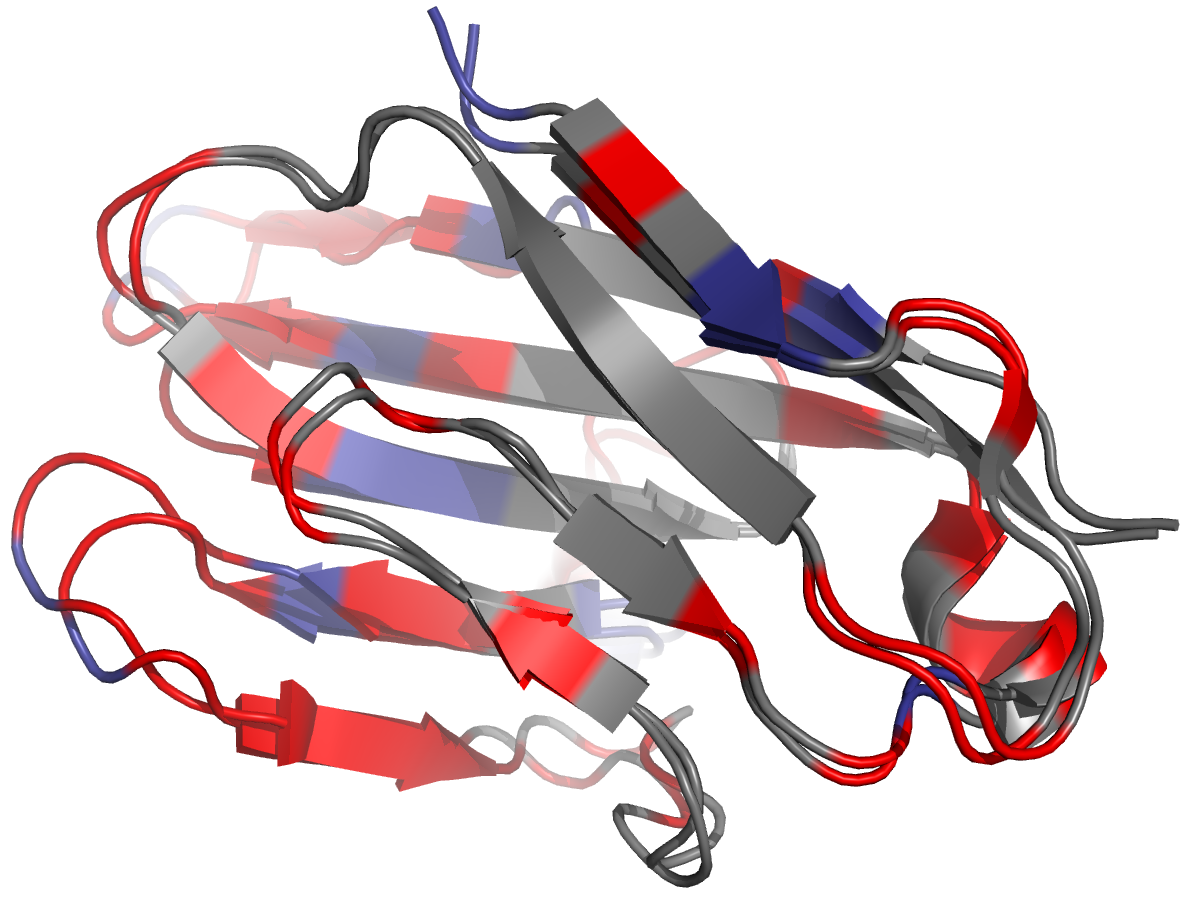
\includegraphics[width=0.58\textwidth]{02-ProtModelling/comparative/comp_42.png}}
}

\mbox{
      \subfigure[Low identity alignment: Alignment of 2GK2A length 111 and 1L6ZA length 107. Alignment yields 45/107 (42\%) identities and 62/107 (58\%)
positives.]{

\begin{minipage}{0.2\textwidth}
\begin{tiny}
\tt %makes the font fixed-width so that all the columns line-up
\begin{tabbing}

\ \ \ \ \ \ \=5\ \ \ \ 10\ \ \ \ \ \ \ \ 20\ \ \ \ \ \ \ \ 30\ \ \ \ \ \ \ \ 40\ \ \ \ \ \ \ \ 50\ \ \ \ \ \ \ \ 60\ \ \ \ \ \ \ \ 70\ \ \ \ \ \ \ \ 80\ \ \ \ \ \ \ \ 90\ \ \ \ \ \ \ \ 100\ \ \ \ \ \ \ \ 111\\\
\>|\ \ \ \ |\ \ \ \ .\ \ \ \ |\ \ \ \ .\ \ \ \ |\ \ \ \ .\ \ \ \ |\ \ \ \ .\ \ \ \ |\ \ \ \ .\ \ \ \ |\ \ \ \ .\ \ \ \ |\ \ \ \ .\ \ \ \ |\ \ \ \ .\ \ \ \ |\ \ \ \ .\ \ \ \ |\ \ \ \ .\ \ \ \ .|\\
2GK2A\ \textcolor{RoyalBlue}{QL}\textcolor{black}{T}\textcolor{red}{T}\textcolor{black}{E}\textcolor{RoyalBlue}{SM}\textcolor{black}{P}\textcolor{red}{FN}\textcolor{black}{VAE}\textcolor{red}{GKE}\textcolor{black}{VLLLVHNLP}\textcolor{red}{QQ}\textcolor{black}{L}\textcolor{red}{FG}\textcolor{RoyalBlue}{YS}\textcolor{black}{WYKG}\textcolor{red}{ERVDG}\textcolor{RoyalBlue}{NRQ}\textcolor{black}{I}\textcolor{red}{VG}\textcolor{RoyalBlue}{Y}\textcolor{red}{AIG}\textcolor{RoyalBlue}{T}\textcolor{red}{QQATP}\textcolor{black}{G}\textcolor{red}{P}\textcolor{black}{A}\textcolor{red}{N}\textcolor{black}{SGRE}\textcolor{red}{T}\textcolor{black}{IY}\textcolor{red}{P}\textcolor{black}{N}\textcolor{red}{A}\textcolor{black}{SLL}\textcolor{red}{I}\textcolor{black}{Q}\textcolor{red}{N}\textcolor{RoyalBlue}{V}\textcolor{black}{T}\textcolor{red}{QN}\textcolor{black}{D}\textcolor{red}{T}\textcolor{black}{G}\textcolor{red}{F}\textcolor{black}{YTL}\textcolor{red}{Q}\textcolor{RoyalBlue}{V}\textcolor{red}{IKS}\textcolor{RoyalBlue}{D}\textcolor{red}{LVNE}\textcolor{RoyalBlue}{E}\textcolor{black}{AT}\textcolor{red}{G}\textcolor{RoyalBlue}{Q}\textcolor{black}{FHVY}\\
\>\textcolor{RoyalBlue}{++}\textcolor{black}{T}\textcolor{red}{\ }\textcolor{black}{E}\textcolor{RoyalBlue}{++}\textcolor{black}{P}\textcolor{red}{\ \ }\textcolor{black}{VAE}\textcolor{red}{\ \ \ }\textcolor{black}{VLLLVHNLP}\textcolor{red}{\ \ }\textcolor{black}{L}\textcolor{red}{\ \ }\textcolor{RoyalBlue}{++}\textcolor{black}{WYKG}\textcolor{red}{\ \ \ \ \ }\textcolor{RoyalBlue}{+++}\textcolor{black}{I}\textcolor{red}{\ \ }\textcolor{RoyalBlue}{+}\textcolor{red}{\ \ \ }\textcolor{RoyalBlue}{+}\textcolor{red}{\ \ \ \ \ }\textcolor{black}{G}\textcolor{red}{\ }\textcolor{black}{A}\textcolor{red}{\ }\textcolor{black}{SGRE}\textcolor{red}{\ }\textcolor{black}{IY}\textcolor{red}{\ }\textcolor{black}{N}\textcolor{red}{\ }\textcolor{black}{SLL}\textcolor{red}{\ }\textcolor{black}{Q}\textcolor{red}{\ }\textcolor{RoyalBlue}{+}\textcolor{black}{T}\textcolor{red}{\ \ }\textcolor{black}{D}\textcolor{red}{\ }\textcolor{black}{G}\textcolor{red}{\ }\textcolor{black}{YTL}\textcolor{red}{\ }\textcolor{RoyalBlue}{+}\textcolor{red}{\ \ \ }\textcolor{RoyalBlue}{+}\textcolor{red}{\ \ \ \ }\textcolor{RoyalBlue}{+}\textcolor{black}{AT}\textcolor{red}{\ }\textcolor{RoyalBlue}{+}\textcolor{black}{FHV+}\\
1L6ZA\ \textcolor{RoyalBlue}{EV}\textcolor{black}{T}\textcolor{red}{I}\textcolor{black}{E}\textcolor{RoyalBlue}{AV}\textcolor{black}{P}\textcolor{red}{PQ}\textcolor{black}{VAE}\textcolor{red}{DNN}\textcolor{black}{VLLLVHNLP}\textcolor{red}{LA}\textcolor{black}{L}\textcolor{red}{GA}\textcolor{RoyalBlue}{FA}\textcolor{black}{WYKG}\textcolor{red}{NTTAI}\textcolor{RoyalBlue}{DKE}\textcolor{black}{I}\textcolor{red}{AR}\textcolor{RoyalBlue}{F}\textcolor{red}{VPN}\textcolor{RoyalBlue}{S}\textcolor{red}{NMNFT}\textcolor{black}{G}\textcolor{red}{Q}\textcolor{black}{A}\textcolor{red}{Y}\textcolor{black}{SGRE}\textcolor{red}{I}\textcolor{black}{IY}\textcolor{red}{S}\textcolor{black}{N}\textcolor{red}{G}\textcolor{black}{SLL}\textcolor{red}{F}\textcolor{black}{Q}\textcolor{red}{M}\textcolor{RoyalBlue}{I}\textcolor{black}{T}\textcolor{red}{MK}\textcolor{black}{D}\textcolor{red}{M}\textcolor{black}{G}\textcolor{red}{V}\textcolor{black}{YTL}\textcolor{red}{D}\textcolor{RoyalBlue}{M}\textcolor{red}{TDE}\textcolor{RoyalBlue}{N}\textcolor{red}{YRRT}\textcolor{RoyalBlue}{Q}\textcolor{black}{AT}\textcolor{red}{V}\textcolor{RoyalBlue}{R}\textcolor{black}{FHVH}\\
\>|\ \ \ .\ \ \ \ |\ \ \ \ .\ \ \ \ |\ \ \ \ .\ \ \ \ |\ \ \ \ .\ \ \ \ |\ \ \ \ .\ \ \ \ |\ \ \ \ .\ \ \ \ |\ \ \ \ .\ \ \ \ |\ \ \ \ .\ \ \ \ |\ \ \ \ .\ \ \ \ |\ \ \ \ .\ \ \ \ |\ \ \ \ .\ |\\\
\>1\ \ \ \ \ \ \ \ 10\ \ \ \ \ \ \ \ 20\ \ \ \ \ \ \ \ 30\ \ \ \ \ \ \ \ 40\ \ \ \ \ \ \ \ 50\ \ \ \ \ \ \ \ 60\ \ \ \ \ \ \ \ 70\ \ \ \ \ \ \ \ 80\ \ \ \ \ \ \ \ 90\ \ \ \ \ \ \ \ 100\ \ \ \ 107\\

\end{tabbing}
\end{tiny}
\end{minipage}
}}

\vspace{0.5cm}

\caption[Sequence:Structure relationships between homologous templates]{Sequence$\to$Structure relationships between typical homologous templates. The sequence alignment
was generated using a PDB  service. Colours in the sequence alignment correspond to those in the structural alignment. Structural images created using \pymolV.
}
\label{fig:intro:seqstrucrelationship}

\end{center}
\end{figure}

So, nature is inherently economical; once a stable protein fold has evolved, the same structural motif is then often reused, augmented with new function.
The implication is therefore that, as long as one can find at least one high-quality representative structure for each of a limited number
of protein folds, the representative member(s) of each fold can be used in the \emph{prediction} of any undefined structures which share high sequence
identity.




\subsubsection{Template Availability}

The future is promising for the scope of available 
modelling templates. \xray\ crystallography is traditionally only applied to proteins of direct interest. However, due to increasing use of template-based
modelling techniques, there has been a recent drive to use targeted high-throughput crystallography to get at least one representative structure for each basic
fold type\cite{COMPCHEM:Gou2002}. This process will inevitably increase the diversity of available templates and allow template-based modelling to be performed on a greater variety of proteins and with a higher degree of accuracy.


\subsubsection{Threading and Fold Recognition}

Fold recognition\cite{SIMULATION:FoldRecognition} and threading\cite{SIMULATION:Threading} methods involve the mapping of sequences onto known protein folds.  The
most recent methods use sequence$\to$structure profiles derived from multiple
sequence alignments in order to enhance
the mapping process\cite{SIMULATION:GenThreader,SIMULATION:Karplus2001}. By scanning fold libraries it is possible to identify structures which are potentially compatible with the target sequence.
This evaluation is performed independent of the sequence identity; only the
energetic stability of a given sequence within a given fold is scored. 
The
most energetically stable folds then progress into further stages of refinement.
Typically, the model represents only the spatially conserved positions of the fold, often the protein core, so the production of an all-atom protein model  requires further stages of surface loop placement and side-chain packing.

Protein threading has a role in protein structure prediction that is intermediate between comparative modelling and \abinitio\ prediction. Using threading, models can be produced for candidate sequences where there
is no high sequence identity template and can often identify the correct
fold; the main problem with these methods is that they often fail to correctly
align the sequence within the fold, resulting in erroneous final models\cite{METHOD:CASP:FoldRecognition}.

\subsubsection{Comparative Modelling}


Comparative or homology modelling is the process by which a 3D model structure is produced, for a chosen candidate sequence, using information
from one or more structural templates which share significant sequence identity. 
Enhancement of comparative modelling is a focus of the work presented in this thesis. The
specific issues in the field of comparative
modelling as a whole are discussed further in section \ref{section:comparative_modelling}
following the introduction of other prerequisite modelling considerations.


\subsubsection{Template-based Modelling Summary}

In summary, template-based modelling provides a shortcut to true \abinitio\ modelling. By effectively tightly pre-defining the topology of the candidate sequence of interest using structural templates, conformational space is vastly reduced and calculation detail can be increased. This not only results
in more accurate models of higher confidence, but also means that models can be generated for larger structures. 

The downside of the use of templates is that structures with novel folds
cannot be predicted. In addition, the models produced by this kind of modelling
say nothing about the pathways, forces and overall energetics of the folding
process itself.
Although template-based modelling will never be a complete solution for \insilico\ protein folding, multi-domain-sized proteins can be modelled using current levels of computer power, making this group of modelling techniques especially
valuable to the molecular biologist.









\section{Protein Representation}
\label{section:protein_rep}

The great dilemma for protein simulation is the balance between the complexity of the protein representation and forcefield used to describe a protein system and the coverage of the conformational search. This balance must be addressed within the scope of available computer power.
Increasing the complexity of the \forcefield, with the aim of increasing its discriminatory power, not only increases the time required to search conformational space, but also usually results in a more difficult search due to the increased number of competing
energy minima. 


The converse is a reduction in the complexity of the protein model, which can reduce the time required to evaluate the chosen scoring functions. This can be accomplished via a reduction in number of particles by using unified residues. For example, the \textsc{Unres}\cite{COMPCHEM:Cza2004,COMPCHEM:Liw97} and \raft\cite{COMPCHEM:Gib2001} representations use centroids to represent the backbone and \sidechain\ atoms. Alternatively, the various \mbox{united-atom}\cite{COMPCHEM:Der99,COMPCHEM:Osg99} representations also aim to reduce the number of particles in the system by amalgamating hydrogen atoms with their parent heavy-atom. Methods accomplishing reduction in conformational space have varied hugely, ranging from simplified coordinate lattice models\cite{COMPCHEM:Hin92,COMPCHEM:Hin94,COMPCHEM:Kol94,COMPCHEM:Cov94} over discretising the allowed values for the conformational variables (such as torsion angles\cite{COMPCHEM:Gib2001}) or by using polypeptide fragment libraries\cite{METHOD:Rosetta,METHOD:Rosetta:CASP3}. \Sidechain\ freedom can also be reduced by using rotamer libraries to represent highly populated conformational sub-states.

The problem with the use of low complexity methods is that oversimplification of protein geometry may severely compromise the specificity required to discriminate between native and non-native compact conformations, especially in the densely packed core regions, and may be partially responsible for the failure of such models with increasing protein size. Equally, over-restriction of backbone geometries may not enable the molecule to fold co-operatively in a way that maximises the attractive energies between interacting bodies, due to the restricted freedom of movement. This could partially account for the significant deterioration in the ability of models with restricted geometry to describe structures which are rich in \bstrands\ in comparison to their representation of \mbox{\al-helical} structure -- The energetic stability of \mbox{\be-structure} is much more sensitive to angle variations\cite{COMPCHEM:Gib2001}.

Continued development of a successful reduced
representation\cite{COMPCHEM:Gib2001} and its application to loop modelling is described further in chapter \ref{chapter:reduced_rep}.
As such representations are incapable of \emph{precisely} representing the native state,
but only native-like states, chapter \ref{chapter:prearcus} goes on to describe the refinement of viable conformations into final all-atom models.






\section{Energy Functions}
\label{section:protmodel:energy_functions}

Protein \forcefields\ play a crucial role in all avenues of protein modelling
including protein dynamics simulations, protein design calculations, modelling
of both protein:protein and protein:ligand interactions and in protein structure prediction. There is a wealth of current research dedicated to improving the ability of protein \forcefields\ to describe the free energy landscape of proteins; signified by a host of recent reviews\cite{FORCEFIELD:REVIEW:1,FORCEFIELD:REVIEW:2,FORCEFIELD:REVIEW:3,FORCEFIELD:REVIEW:4}.

Each of these simulation classes is clearly attempting to model the same underlying
physical laws, therefore theoretically, if infinite computer power were available, a single perfect \forcefield\ would be sufficient for all protein simulation. Critically however, computer power is finite and so, depending on the specifics of a given simulation, the chosen \forcefield(s) must strike the optimal balance between calculation detail and speed. For example, a docking
\forcefield\ is required to rapidly screen many millions of small compounds \insilico\ and therefore favours speed of execution. Even the most detailed docking \forcefields\ are usually only concerned with soft-sphere sterics, crude empirical hydrogen bonding and  desolvation terms within the active
site. By contrast, to make predictions of physical quantities like   folding rates, detailed protein folding simulations  are required. These  must employ the highest quality physical models and use  explicit solvent at the expense of calculation speed. 

Forcefields for protein structure prediction reside between these two poles.
The crucial difference is that these algorithms are not required to simulate
protein kinetics, but are instead required to distinguish between a  number of distinct
conformational states. The chosen \forcefield\ is typically required to screen many thousands of these potential protein models, but also needs to describe the native state with sufficient clarity to discriminate against protein-like competing minima.



It is important that the chosen forcefield successfully models, directly or indirectly, the hydrophobic effect, electrostatics, solvation effects and hydrogen bonding.
 Frequently in protein modelling, forcefields based upon statistical potentials, derived from the PDB, or simplified physico-chemical \forcefields\ are used. Molecular mechanics \forcefields,  particularly when augmented with implicit solvation models, provide increasingly successful physics-based energetic evaluations. Historically they have not been extensively used, due to their relative computational expense, but are now beginning to play an  important role.

\subsection{Molecular Mechanics Forcefields}

In a traditional molecular mechanics \forcefield, the potential energy of the system is broken down into a defined number of individual components. The sum of
these components is  used to represent the energetics of each competing conformation on the folding landscape. 

Equation \ref{eqn:intro:mmff:A} shows how the energy of the system is split between bonded and non-bonded terms.
Each of the terms shown is usually referred to as a potential energy function,
or PEF, as they aim to describe the potential as opposed to the kinetic energy
of the system. The parameters for the the various PEFs of molecular mechanics
forcefields are derived from many sources including both quantum mechanical calculations and thermodynamic, crystallographic and spectroscopic data for a wide range of systems\cite{FORCEFIELD:REVIEW:3,FORCEFIELD:REVIEW:4}.

\begin{equation}
\Delta E_\mathrm{System} = \Delta E_\mathrm{Bonded} + \Delta E_\mathrm{Non-Bonded}
\label{eqn:intro:mmff:A}
\end{equation}

The most popular ``Third Generation'' molecular mechanics forcefields are \amber\cite{FORCEFIELD:AMBER,COMPCHEM:Pon2003},
\charmm\cite{FORCEFIELD:CHARMM}, \textsc{Opls}\cite{COMPCHEM:OPLS,COMPCHEM:OPLS:B} and \textsc{Gromos}\cite{COMPCHEM:GROMOS}. Each implementation is based on the
same broad principles but varies in its specific details. These are all available in multiple versions and differing atomic detail.

\subsubsection{Bonded Energy Terms}
\label{section:protmodel:bondedterms}

Equation \ref{eqn:intro:mmff:B} shows the standard bonded \forcefield\ terms
which are concerned with the geometry of covalently linked atoms. Unfavourable energy is associated with deviations from optimal molecular geometry. Bond lengths, angles between bonded atoms and torsion angles along each bond are all constrained near populated equilibrium values using separate PEFs. 

Each covalently linked atom pair is joined by a bond; the energetics of 
which are usually
approximated
using a simple harmonic potential with an associated force constant. Each angle between these bonds
is also harmonically
restrained  to a given equilibrium value. Torsions on the other hand are modelled using a periodic function which aims to model the energetic barriers found during bond rotation. 

Bonded energies vary greatly with even small deviations away from equilibrium
values and are therefore meaningless unless a given protein conformation
is first locally energy minimized. As a simplification, some algorithms choose to work only with idealised geometry and therefore can completely ignore
both the bond and angle terms.

\begin{equation}
\Delta E_\mathrm{Bonded} = \Delta E_\mathrm{Bonds} + \Delta E_\mathrm{Angles} + \Delta E_\mathrm{Torsions}
\label{eqn:intro:mmff:B}
\end{equation}

\subsubsection{Non-Bonded Energy Terms}

Equation \ref{eqn:intro:mmff:C} defines
the non-bonded \forcefield\ terms, which are concerned with the interactions between atoms which are not covalently linked. These  PEFs  usually include
both the Lenard-Jones potential and Couloumbic interactions.
In order for the aqueous solvent to be represented without explicitly modelling water molecules, implicit solvent terms are often included to define solvent interactions. 

\begin{equation}
\Delta E_\mathrm{Non-Bonded} = \Delta E_\mathrm{Lenard-Jones} + \Delta E_\mathrm{Coulombic} + \Delta E_\mathrm{Solvation}
\label{eqn:intro:mmff:C}
\end{equation}

The Lennard-Jones potential, given in equation \ref{eqn:intro:mmff:lj}, aims to represent both weakly attractive \vdw\ (VDW)  forces and the strongly repulsive forces caused by orbital overlap. $\epsilon$ and $\sigma$ in this case are atom-dependent parameters. The functional form of the Lenard-Jones potential is very sensitive to atomic
radius overlap. This is sometimes replaced
by a soft-sphere alternative, which is more forgiving during protein simulation.

\begin{equation}
\Delta E_\mathrm{Lenard-Jones} = 4 \epsilon \left[  \left( \frac{\sigma}{r} \right)^{12} - \left( \frac{\sigma}{r} \right)^{6} \right]
\label{eqn:intro:mmff:lj}
\end{equation}

Couloumbic or 
electrostatic interactions are usually described by Coulomb's law using equation \ref{eqn:intro:mmff:couloumb}, in which  $\epsilon_0$ is the permittivity of free space, $\epsilon$ is the dielectric constant, $r_\mathrm{ij}$ is the separation of atoms $i$ and $j$ in angstroms and $q_i$ and $q_j$ are charges of atom $i$ and atom $j$ respectively.

\begin{equation}
\Delta E_\mathrm{Coulombic} = \sum^N_\mathrm{i=1} \sum^N_\mathrm{j=i+1} \frac{1}{4 \pi \epsilon_0 } \frac{q_iq_j}{r_\mathrm{ij}\epsilon}
\label{eqn:intro:mmff:couloumb}
\end{equation}

In the context of protein modelling, bonded forcefield terms can be satisfied by many different protein conformations.
 The real discriminatory power of a \forcefield\ must be derived from the treatment of hydrogen bonding, long range electrostatic effects and the highly complicated effects of solvent interaction. Protein modelling  is therefore critically linked to the representation of the electrostatic and solvation components of the forcefield.
The ultimate  driving force of the non-bonded components is to produce compact protein structures in a way that also satisfies molecular geometry.    

Modern molecular mechanics PEFs model hydrogen bonds within the careful balance
between the electrostatic and and Lennard-Jones interactions. Some alternatives
 implementations\ utilise specialised hydrogen bonding terms which can involve \emph{explicit} directional specificity.

\subsubsection{Implicit Solvation}
\label{section:protmodel:implicit_solvation}

Real globular proteins, of course, reside permanently within aqueous solvent. Good
atomic models for water, termed explicit solvent, do exist and are commonly used in high-detail MD simulations. Explicit solvent however poses a number of difficulties for protein structure prediction algorithms. Firstly, \forcefield\ calculations often involve pairwise comparisons between all atoms in the
system. If water is included
in the simulation  it introduces a large number of additional atoms and in
turn hugely increases the number of pairwise calculations.
Secondly, some prediction algorithms utilise  large changes in the protein conformation, meaning that after each move, the water must be re-equilibrated in order to make an energy calculation. Finally computing the energy of a protein embedded in explicit
solvent molecules is time consuming, because the energy
must be averaged over many solvent configurations. All these problems are avoided by treating the solvent as a time-averaged continuum, also known as an implicit solvent model. 

Equation \ref{eqn:intro:impsol} describes the basis of the implicit solvation model whereby the solvent is modelled as a continuous bulk property. The energetics between the protein and the solvent continuum are usually divided into two components. 

\begin{equation}
\begin{array}{ll}
\Delta E_\mathrm{Solvation} 
& = \Delta E_\mathrm{Vacuum \to Water} \\
& = \Delta E_\mathrm{Polarisation} + \underbrace{ \Delta E_\mathrm{VDW} + \Delta E_\mathrm{Cavity}}_{\mathrm{Surface~term}}
\\
& \approx \Delta E_\mathrm{Polarisation} + \displaystyle \sum^n_\mathrm{i=1} \sigma_i
\mathrm{SASA}_i \\
\end{array}
\label{eqn:intro:impsol}
\end{equation}

$\Delta E_\mathrm{Polarisation}$ is the solvation polarisation energy which accounts for the interaction of the partial charges
within the protein and dipoles which these charges induce within the bulk
solvent. The result of this is that atomic charges closer to the protein surface are more favourable and show weaker apparent charge-charge interactions with each other. The solvation polarisation energy is usually calculated using the generalised Born method and describes interaction of atomic charges.
The usual formulation of this PEFs is described further in the following section.

$\Delta E_\mathrm{VDW} + \Delta E_\mathrm{Cavity}$ accounts for the hydrophobic effect, describing the interfacial free energy of uncharged protein with the solvent continuum. The surface term consists of two basic components. The first is the favourable VDW interaction energy with the solvent. The second is an unfavourable cavity term which calculates an entropic cost for ordering solvent at the solute$\to$solvent interface upon the formation of the solvent cavity. It is assumed that these effects are strongest on the first shell of water around the solvent and therefore the energy would be proportional to the solvent-accessible surface area (SASA)\cite{FORCEFIELD:SASA}. For each atom ($a_i$), the surface constant $\sigma_i$
is  multiplied by $\mathrm{SASA}_i$ in the calculation.
Alternative pairwise methods are available which are computationally
more efficient but give less accurate results\cite{FORCEFIELD:POPS}.

 
\subsubsection{The Generalised Born Formulation}
\label{section:intro:gb}

In implicit models, the solvent is usually treated as a time-average
continuum with bulk solvent properties. The electrostatic interactions of a protein in solvent
are modelled as a set of point charges,  placed inside a low-dielectric cavity, surrounded
by a high-dielectric medium. In such a model, the Poisson-Boltzmann (PB) equation (\ref{eqn:intro:poisson})
relates the electrostatic potential ($\phi$) and the dielectric constant vector (r).   $\nabla$ (dell)\ is the differential operator.

\begin{equation}
\nabla.\epsilon\left(r\right)\nabla\phi\left(r\right)=\rho\left(r\right)
\label{eqn:intro:poisson}
\end{equation}

The PB equation, for all but the simplest systems, must be solved numerically 
via the finite difference method.
This places point charges and their associated radii of influence on a grid of finely spaced points, where the finer the grid, the more accurate the end result. This numerical technique makes any calculations using the PB equation
intrinsically slow.
The generalised Born\cite{FORCEFIELD:GB} (GB) model has recently received considerable attention as a rapid approximation to the numerical solution of the PB equation. Because the GB model is intrinsically based on the same underlying continuum approximation as used in PB theory, its accuracy is naturally assessed by comparison with the PB results. 

The GB model calculates the electrostatic polarisation free energy caused
by the movement of a protein solute into aqueous medium. This involves a change in the inherent polarisability of the medium, \ie the ability for the molecules to align themselves with the reaction field. This is described by a dielectric value ($\epsilon$), which accounts for the shielding of electrostatic interactions in the protein solute. As the protein moves from vacuum \mbox{($\epsilon$=1)} to aqueous solvent \mbox{($\epsilon$=80),} electrostatic effects within the solute become weaker.
The protein solute dielectric constant is poorly defined and has been assigned values between 1 and
20, although values between 2 and 4 are most common.

\begin{figure}[hptb]
\begin{eqnarray}
\Delta E_\mathrm{Polarisation} = -\left( 1 - \frac{1}{\epsilon} \right)
\sum^N_\mathrm{i=1} \sum^N_\mathrm{j=i+1} \frac{q_iq_j}{f_\mathrm{GB}}
 - \frac{1}{2}\left( 1 - \frac{1}{\epsilon} \right) \sum^N_\mathrm{i=1} \frac{q^2_i}{a_i}
\label{eqn:intro:gb} \\
f_\mathrm{GB} = \sqrt{ r^2_\mathrm{ij} + a_i a_j \exp{ \left( \frac{-r_\mathrm{ij}^2}{4a_ia_j} \right) } }
\label{eqn:intro:gb3}
\end{eqnarray}

\begin{tabular}{ll}
Where,&\\
$N$ & The total number of atoms \\
$\epsilon$ & The effective solute dielectric \\
$r_\mathrm{ij}$ & The separation of atoms i and j (\AA) \\
$q_i$ and $q_j$ & The charges of atom i and atom j respectively \\
$a_i$ and $a_j$ & The effective Born radius of atom $i$ and $j$ respectively\\
\end{tabular}

\caption{The formulation of the generalised Born equation}
\label{fig:intro:gb}

\end{figure}

The GB equation (\ref{eqn:intro:gb}) itself  has two components. The first term describes the reduction in electrostatic
energy as you move from vacuum to a dielectric medium. The second term is the favourable
energy that the system gains as its charges interact with their own induced field in the high dielectric medium. The Born radius applies to a point charge sitting at the centre of a perfectly spherical cavity whereas the effective Born radius, first introduced by Still et al.\cite{COMPCHEM:Still90}, is used for charges within non-spherical cavities. The effective Born radius of a point charge in a non-spherical cavity is equal to the Born radius of an identical ion, with the same charge and polarisation energy, in a spherical cavity. The exact methods to calculate effective
Born radii are beyond the scope of this discussion, but in essence a GB calculation using perfect effective Born radii for each atom in a given solute, will yield a very close approximation to the result of a fine-grid finite-difference PB calculation.
A host of recent advances in the precise formulation \cite{COMPCHEM:Tsu2000,COMPCHEM:Bas2000,COMPCHEM:Sim2001,FORCEFIELD:GB:ADVANCES:A,FORCEFIELD:GB:ADVANCES:B} have
resulted in GB solvation energies that now correlate extremely well with PB energies\cite{FORCEFIELD:PBGB:COMPARE}.



\subsubsection{Current Success}

Even the third generation molecular mechanics forcefield implementations, such as \ambergbsa, are still not truly reliable. It is certainly true that conformations are often found which are lower in energy than the experimentally defined native state\cite{METHOD:Plop}  and that current forcefields cannot always distinguish between native-like and protein-like decoy structures. In order to distinguish native-like conformations during protein simulation, future molecular mechanics \forcefields\ must become even more detailed, probably more extensively using quantum mechanical calculations for parametisation, although those methods are by no means mature at this stage.


\subsection{Knowledge-based and Statistical Energy Functions}


 Statistical \forcefields\ are typically derived from structural data within the
PDB. Geometric quantities and contacts are measured to obtain frequency distributions
which are averaged to derive pseudo-potentials, also known as potentials of mean force (PMFs). Commonly a single effective interaction site is chosen
for each residue, which is usually the \ca\ or \cb\ atom, from which distances
to other interaction sites are measured\cite{FORCEFIELD:REVIEW:KNOWLEDGEBASED}.

The principle advantage of statistical potentials is their raw speed. Compared
to full molecular mechanics \forcefields, even complex statistical potentials are at least an order of magnitude faster. The complementary disadvantage of statistical potentials is their great freedom of functional form causes
a highly tentative relationship to free energy. Crucially, statistical potentials derive from the finite PDB, which by its nature is a snapshot of the protein structures which are experimentally amenable.\
The PDB therefore is unlikely to accurately reflect all protein structures in nature.

One must be extremely careful not to introduce artifacts into the overall statistical potential. Many knowledge-based potentials completely disregard the context of each given
residue$\to$residue interaction.  An example of this would
be the naive observation that like-charged aspartic acid residues are found
in close proximity. Closer observation would reveal that the majority of
this probability density stems from the fact that aspartic acid residues
are frequently found in coordination with strongly positive metal ions. Thus
the interaction energy of these two \sidechains\ is required to be very different
between a metal and non-metal binding context. The issue of context is also
important for some rare, but strong interactions found in very specific contexts.
Such low-frequency observations would be given an unfavourable energy by
statistical potentials even though they are perfectly valid states. More
recent implementations attempt to remedy these issues by utilising sequence
similarity to select between multiple sets of derived potentials\cite{FORCEFIELD:Skolnick2000}.

In spite of all this, database potentials have been shown to be effective at discriminating between correct and incorrect model structures. It has also been shown that the best knowledge-based forcefields can reproduce physical quantities such the likelihood of a residue to be buried\cite{COMPCHEM:DFIRE}.



\subsection{Simplified Physico-Chemical Forcefields}

For coarse-level simulation of protein folding, it can be appropriate to
use heavily cut-down forcefields which are still based on underlying physical
principles. These physico-chemical forcefields attempt to approximate, to
varying extents, the fundamental forces between atoms and groups within the
protein. 

It is generally found that the hydrophobic effect alone is insufficient to
find protein-like conformations of small proteins. By including both hydrophobic
and polar pair-wise potentials, however, some success has been found in the
discrimination of native from non-native conformations\cite{FORCEFIELD:Huang95}. Further success has been found in the use of backbone hydrogen bonding potentials\cite{FORCEFIELD:Lee1996}. A comparatively more complex method uses similar hydrophobic and hydrogen bonding
functions with additional molecular mechanics style bonded potentials\cite{FORCEFIELD:Wallqvist1994},
however this additional level of complexity somewhat goes against the purpose
of such a reduced forcefield.



\subsection{Comparing Molecular Mechanics and Statistical Potentials}

Molecular mechanics and statistical \forcefields\ have clear advantages and
disadvantages and are ultimately suited to different roles within different
protein modelling applications. An example of where simplified physico-chemical
and statistical potentials are far more suitable is in discrimination between un-optimised structures, as molecular mechanics forcefields are exquisitely
sensitive to small changes in atom positions. Even small atomic overlap in
a given non-energy-minimised model will result in any molecular mechanics forcefield producing a meaningless energy evaluation.

The ultimate test of these very different styles of \forcefield\ is to test
them against each other, with an emphasis on the ability to distinguish between correct and incorrect structures. Recently, the \charmm\ molecular mechanics forcefield and a statistical potential
were compared for a range of conformations of the GCN4 leucine zipper\cite{FORCEFIELD:Mohanty1999}.
The study found excellent correlations both between the two forcefields and the
RMSD of each conformation to the native conformation. Neither forcefield
however identified the native state as the lowest energy conformation.

It is usual for statistical potentials to be described with somewhat arbitrary
mathematical representations which are computationally efficient and facilitate rapid calculations. Molecular mechanics \forcefields\ score protein
conformations in real units of enthalpy, by contrast statistical potentials
by nature must score based upon the frequencies of occurrence of structural
features found within high-resolution proteins structures. These frequencies
are then interpreted as free energies by assuming that the Boltzmann hypothesis\cite{FORCEFIELD:Shortle2003}
holds true, a practice that is not agreeable to all\cite{FORCEFIELD:REVIEW:KNOWLEDGEBASED}. 

An additional issue
that is related to simulation of the folding landscape is that  statistical
potentials are derived from compact folded proteins and therefore will
not be effective in representing the energetic interactions along the folding
pathway. By contrast, molecular mechanics \forcefields\ have the advantage of resting on a clear theoretical basis, allowing an in-depth analysis of energetic contributions to folding. A caveat to this is that current molecular mechanics
forcefield implementations utilise simplifications which are  necessary for tractable computing. Following further development and advances
in computer capacity, theoretical detail can be increased, thus allowing some
of these underlying simplifications to be removed. This should result in an improvement
in the discriminatory capacity of such \forcefields. 





\section{Searching Conformational Space}
\label{section:protmodel:conformational_search}

An exhaustive conformational search is impossible for all but the simplest model systems, hence
in order to find energy minima, an effective non-exhaustive search method is  required.
There are three main classes of search method, where each contains many sub-classifications:

\begin{itemize} \isep
\item 
Deterministic algorithms include build-up procedures.
Deterministic algorithms have a defined solution, thus given a particular input, they will always produce the same output.
\item
Stochastic algorithms include Monte Carlo (MC), replica
exchange, branch-and-bound and simulated
annealing. Stochastic algorithms are often faster than deterministic alternatives, however, they may return sub-optimal results.
\item
Heuristic algorithms include genetic algorithms. In general, a heuristic is a ``rule of thumb'' that guides the selection of a set of candidates at each stage of a search process. \\[-0.9cm]
\end{itemize}

If information on the dynamics of folding is required, then conceptually either MD or  MC with small conformational moves can allow the polypeptide to follow a folding pathway.
Each of these methods are briefly discussed in the following sections.

Search frustration is defined here as calculation-time spent re-exploring
the energy well of a single local minimum. The level of frustration is closely related to two important aspects of each search method.\ The first is the type and scale of conformational moves which are made to the system. Too small and the system will become frustrated, too large and nonsense structures will frequently be generated. The second aspect is
the technique which is used to escape
frustration during the search.  These aspects are discussed
in the remainder of this section where appropriate.

 

 

\subsection{Build-up}

Build-up procedures   function by joining successively long pairs of 
 polypeptide chain fragments, beginning from a single residue\cite{SIMULATION:BUILDUP}. At each stage of joining all combinations of the minima for each fragment are tested. Each fragment combination is screened for high-energy and steric overlap and subsequently minimised in \phipsi\ space. Highly similar fragments are removed to reduce redundancy. As the algorithm progresses, the chain increases in length, hence the term build-up. Such methods have been criticised
for not treating the protein as a whole during the early stages of structure
generation.

 
\subsection{Monte Carlo}

Monte Carlo (MC) searches involve pseudo-random sampling of the potential
energy surface\cite{SIMULATION:MC}. By applying a number of different types of conformational perturbations such as torsions, Cartesian coordinates, \sidechain\
rotamers as well as other more specialised moves, the conformational space
of the polypeptide chain may be explored. 

In simple MC, conformational changes are only kept if they result in an energetic
improvement.  In a system such
as protein modelling, many competing local minima exist and therefore the
conformational search is easily frustrated. This makes simple MC intrinsically inefficient, however, some common improvements which vastly improve the search process are outlined below.  

\subsubsection{The Metropolis Criterion}

The Metropolis Criterion\cite{SIMULATION:Metropolis}, shown in equation \ref{eqn:intro:metropolis}, is
used to relieve frustration in the MC\ search process by allocating a probability
that conformational changes can be made which result in an \emph{increase} in energy.
The formalism defines that decreases in energy are always accepted, whereas
an increase may be accepted at random, dependent on the Boltzman constant
($k_e$),
the magnitude of the energy increase ($\Delta E$) and the temperature of the system ($T$).
The end result is that jumps between competing local minima are more likely
as higher energy \emph{intermediate} structures may be visited.

 
\begin{equation}
P_\mathrm{accept} = \left\{ \begin{array}{ll}
 \Delta E \ge 0
  & exp^{ \left( \displaystyle \frac{- \Delta E}{k_eT} \right) } \\
\Delta E < 0
  & 1 \\
\end{array}
\right.
\label{eqn:intro:metropolis}
\end{equation}

\subsubsection{Simulated Annealing} 

Simulated annealing\cite{SIMULATION:SimulatedAnnealing} was originally formulated
as an extension to general MC, but can be utilised in all simulations where
some manner of temperature is included. The basic principle is that if
a hot dynamic system is cooled infinitely slowly to absolute zero it will cool to
the global minimum. By  cooling slowly enough, usually multiple times, possible
low energy minima can be found.


\subsubsection{Stochastic Tunneling}
\label{section:protmodel:stun}

Stochastic tunneling, or STUN\cite{SIMULATION:STUN}, aims to circumvent the slow dynamics of ill-shaped energy functions  by tunneling through energy barriers. It accomplishes this by modifying the acceptance function of standard MC  using a nonlinear
transformation to the potential energy surface. All energy wells that lie above the best minimum found so far are suppressed, so that when the simulation escapes the current well, it will not be trapped by local minima that are higher in energy. Energy wells with deeper minima are both preserved and enhanced.

 
The mathematical formalism of the STUN transform is shown in equation \ref{eqn:intro:stun},
where $f$ is the energy of the current conformation, $f_0$ is the lowest minimum encountered thus far and $\gamma$ is a
scaling factor which controls the steepness of the
transformation. 
\begin{equation}
f_\mathrm{STUN}(x) = 1-exp \left(  -\gamma(f( x) -f_{0} \right)
\label{eqn:intro:stun}
\end{equation}

STUN has been used to successfully predict
the structure of the TrpCage mini-protein\cite{SIMULATION:STUN:trpcage}.


\subsubsection{Replica Exchange}

Replica exchange, also known as parallel tempering, improves the dynamic properties of MC simulations of physical systems and is also
applicable to molecular dynamics\cite{SIMULATION:REMD}. In such
algorithms, multiple simultaneous simulations are run at different ``temperatures'',
the higher the temperature the higher the probability of making changes which
increase the energy of the system. The replica exchange occurs when the conformations
are swapped between different temperatures. In the simplest case two parallel
simulations are used where the high temperature effectively causes large deviations in conformation and the low temperature simulation is responsible for exploring around the local energy minima. By recording the low-energy minima throughout the simulation, the global
minimum of the system can potentially be found. Through careful selection of both
temperatures and number of replicas an improvement in the mixing properties of a set of MC simulations can be achieved. This provides sampling efficiency
improvements that exceed the additional computational cost of running multiple parallel simulations.




\subsection{Branch-and-Bound}

In branch-and-bound algorithms conformational space is partitioned by a quantity
such as the backbone \phipsi\ angles or inter-residue distances. For each partitioned region of space, a range of candidates are generated and screened, from which a number of areas of conformational space can be eliminated. From this selection of candidates, more potential structures can be generated. By iteratively repeating this process large regions of conformational space can be eliminated,
removing it from the search scope and increasing the efficiency of the search
process. It is critical that the method of partitioning  conformational space and
the criterion for exclusion are carefully chosen so that they do not exclude a path that will lead to the
global minimum.
It was found in a recent branch-and-bound publication that the method can
potentially be more efficient than standard Monte Carlo at finding the global energy minimum\cite{SIMULATION:BranchAndBound}.

\subsection{Genetic Algorithms}

Genetic algorithms are based on the well defined genetics  doctrine of the
evolution of species via the survival of the fittest. The method begins by the generation of a host of  different conformations, by random means or otherwise, but with significant structural diversity. These conformations are then screened for fitness via an energy criterion and a proportion are retained. These are then mutated to generate a series of children for each conformation. In true genetic algorithms there is also crossover between parent structures.
By iteratively repeating this process, multiple low energy conformations
can be generated. Genetic algorithms have had success both for generation of native-like structures for short peptides\cite{COMPCHEM:Gib2001,SIMULATION:Genetic} and helical bundles\cite{SIMULATION:Genetic:HBundle}.

Genetic algorithms become Memetic algorithms when, as part of the algorithm,
some sort of local conformational optimisation is included prior to selection of the next generation. Such local optimisation has been shown to give greater
efficiency than a standard genetic algorithm\cite{SIMULATION:Memetic}. 




\subsection{Molecular Dynamics}

Protein structure prediction is commonly unconcerned with the dynamics and
pathways of the  folding process. If such properties are required, then simulations
of protein
dynamics must be performed. The usual manner of obtaining such information
is Molecular Dynamics (MD) which simulates individual atoms using
Netwon's laws of motion.

Previous work suggests that short molecular dynamics simulations have only limited use in convergence towards the experimental structure \cite{NATIVE:Venclovas1999}.
Simulations must sample enough of the conformational space to ensure that energetic minima are found. Ergodic theory, which is assumed to be applicable to molecular dynamics, relates to the long-term behaviour and properties of dynamic systems. The theory states that if a system is sampled for a sufficient time, all the possible states of the system will be visited. An adequate duration of sampling is consequently of high importance. 

To give an idea of the required computer power, a recent high-publicity molecular dynamics simulation on the Villin Headpiece (36 amino acids) in implicit
solvent of only 1$\mu$s of folding time took $\sim$2 months CPU time on a 256-CPU Cray Supercomputer\cite{COMPCHEM:Kol98}.
Since this time, simulations of the TrpCage mini-protein (20 amino acids) have been performed
in full explicit solvent\cite{SIMULATION:TRPCAGE:EXPLICIT}. This and other recent high detail simulations can now obtain measurements in agreement
with the Nuclear Overhauser measurements obtained in NMR experiments\cite{SIMULATION:TRPCAGE:IMPLICITNMR}.
Molecular dynamic of large systems is also possible over shorter timescales. At the time of writing, some of the most impressive simulations possible are an incredible 50ns simulation of an entire satellite tobacco mosaic virus in explicit solvent totalling over 1 million atoms\cite{SIMULATION:STMV} and a 2.64 million atom simulation of the ribosome\cite{SIMULATION:Ribosome}.

Today,  bio-simulations of the protein folding process itself are only a realistic prospect for sub-domain sized chains. Significant advances have been made in the last few years and simulations are increasingly being shown to be capable of quantitative predictions such as the folding rate of a given polypeptide\cite{SIMULATION:Snow05}.
Insights into  the physical process of protein folding will ultimately come from these protein folding pathway simulations and will facilitate identification of both transition states and folding intermediates, some of which will prove to be functionally important.





  
\subsection{Conformational Space: Final Comments}

Conceptually search methods which use large conformational shifts disregard any contribution that the folding pathway itself has in determining the native
state. A theoretical issue would be if the global minimum of the system was inaccessible to the polypeptide chain during folding, but could be visited by a large artificial conformational shift during simulation. 

As has been discussed, the native state is likely to be the global free energy minimum, although conceptually this may not be the case. It is impossible, both \insilico\ and \invivo, for a polypeptide to sample
the entirety of conformational space. It is, therefore, likely that \invivo\ folding is directed by local interactions, biasing
the populations within unfolded ensemble. This implies that the native state is a deep and defined minimum, close to that of the biased unfolded ensemble.

It is also true that, given time \invitro, both amorphous aggregates and amyloid fibrils form spontaneously in protein solutions; so these competing
states must be low in free energy. Evolutionary pressure
is likely to favour polypeptide sequences which exhibit high energy
barriers to these    
 states, as they impair the activity of the cell.  Crucially, therefore, it
is likely that these states are further from the unfolded ensemble
 in conformational space, and therefore are not visited within folding timescales. 

\al-lytic protease is an interesting isolated case where, following post-translational
processing
of the polypeptide chain,  the folded state is a actually \emph{higher} in free energy than the unfolded state\cite{NATIVE:unfolded:lowerenergy}. This
case, however, does \emph{not}  break the thermodynamic hypothesis, as it is the pre-processed
state
of \al-lytic protease
is still lower in free energy than the native ensemble.
It appears that a large energetic barrier to un-folding exists for the post-processed chain, being kinetically trapped by the post-processing event and giving it  its apparent stability. This can be shown experimentally,
as
if the post-processed form is unfolded \invitro, it no longer spontaneously
refolds when folding conditions are restored.






 



\section{Comparative Modelling in Detail}
\label{section:comparative_modelling}


Comparative modelling was traditionally performed by expert human modelers whereby
the  alignment of a candidate sequence to a chosen structural template  would be manually optimised. Individual residue
mutations and packing would be performed by eye using visual tools such as
\textsc{Accelrys' Insight II}~hosted on expensive Silicon
Graphics workstations. Such expert-based modelling is often augmented by
 the appropriate use of fragment stitching tools to aid surface loop prediction; implemented in applications such as \textsc{Swiss-PDBViewer}\cite{METHOD:SWISSPDB:A,METHOD:SWISSPDB:B}. Manual modelling is
however extremely labour intensive and hinged critically on correct human judgement.

The advent of more automated responses to the modelling process  has had
a profound impact on structure prediction. When suitable templates
are available such methods are commonly
among the most successful during the modelling competition \casp\cite{METHOD:CASP6:CM}. Modern
comparative modelling utilises these automated processes, guided by human
experts where sequence identity is low. 


\subsection{Archetypes for Automated Comparative Modelling}
\label{section:protmodel:comparativemodellingarchetypes}


All comparative modelling methodologies utilise one or more structural templates at their
heart. The exact method   for structure building however varies between different
implementations. In general, all comparative modelling methodologies are not only extremely rapid, but also do not
\emph{require} human intervention (although this is still entirely possible),
and most give quantification of the certainty
of each region in the final model. 

There are three archetypal implementations
of comparative modelling:
\begin{description} \isep
\item[Rigid-body Assembly] \eg \textsc{Composer}\cite{METHOD:COMPOSER} \\
The first and still widely used approach in comparative modelling is to assemble a model from a small number of rigid bodies obtained from aligned template structures. The approach is based on the natural dissection of the protein structure into conserved core regions, variable loops that connect them and \sidechains\ that decorate the backbone. First, the template structures are selected and superimposed. Second, the ``framework'' is calculated by averaging the coordinates of the \ca\ atoms in structurally conserved regions of the template structures. Third, the backbone atoms of each core region in the target model are obtained by superposing on the framework the core segment from the template whose sequence is closest to the target. This is followed by surface loop and \sidechain\ modelling.

\item[Segment Matching] \eg \textsc{Segmod}\cite{METHOD:SEGMOD} \\
The basis of modelling by coordinate reconstruction is the finding that most hexapeptide segments of protein structure can be clustered into just 100 structurally different classes\cite{METHOD:Unger1989}. Thus, comparative models can be constructed by using a subset of atomic positions from conserved regions of the template structures as ``guiding'' positions (usually \ca), and by identifying and assembling short, all-atom segments that fit these guiding positions. The segments are obtained in a representative database of all known protein structures\cite{METHOD:SEGMOD}.

\item[Satisfaction of Spatial restraints] \eg \modeller\cite{METHOD:MODELLER}
\\
This group of methods work by minimising global deviation from a set of spatial constraints. In \modeller\ these constraints (what it terms probability density functions, or PDFs) are derived from both idealised atomic geometry (obtained from the \textsc{Charmm22}\cite{FORCEFIELD:CHARMM,COMPCHEM:MacKerell1998} molecular mechanics forcefield) and homology derived restraints (distance and dihedral angle restraints) from a statistical analysis of relationships to the template structures. This system assumes that the corresponding distances between aligned residues in the template and the target structures are similar, which is why residue correspondence in the initial sequence alignment must be correct. The allowed range of values of distance or dihedral angle deviation depends on the degree of structural variability at the corresponding position in the template structures. In the final stage approximate 3D models are refined by restrained molecular dynamics with simulated annealing in water.

\end{description}




Modelling by satisfaction of spatial restraints, is generally deemed to be the most successful of the methods. The particular strength of  restraint-satisfaction methodologies is that restraints, empirically weighted by certainty, can be derived from many diverse sources. Such sources include homology-derived restraints,
rules for secondary structure packing\cite{METHOD:Coh89}, analyses of hydrophobicity\cite{METHOD:Asz94}, correlated mutations\cite{METHOD:Tay94}, empirical potentials of mean force\cite{METHOD:Sip90}, cross-linking experiments, NMR data\cite{METHOD:COMPOSER}, image reconstruction in electron microscopy and site-directed mutagenesis\cite{METHOD:Boi93}. This allows as much information as possible to be incorporated into the final ensemble of models. These should all be compliant with all known experimental data and with more general knowledge about protein structure.



\subsection{Web-based Comparative Modelling}

As comparative modelling has become increasingly popular, many modelling programs have been converted into automated
internet-based servers. These include \textsc{Swiss-Model}\cite{METHOD:SWISSMODEL},
\textsc{3D-Jigsaw}\cite{METHOD:3DJIGSAW} and \esypred\cite{METHOD:Esypred3D}
which uses \modeller\ as its internal structure generation engine and augments
it with superior sequence alignment. 

These servers greatly simplify the modelling
process, making it accessible, even to those with limited computer experience. The caveat of this is that simulation detail must therefore be compromised in order to provide a publicly available high-throughput server
which can produce models rapidly on demand. A more accurate model can potentially be generated if a more exhaustive systematic process is utilised off-line;
for example a greater number of surface loops could be sampled, or multiple alternative alignments could be attempted. 


A recent trend that has emerged since \casp-6 is the advent of the consensus server\cite{METHOD:CASP6:CM}. This new class of server interrogates multiple modelling servers for
a given candidate sequence. As all the different servers rely on difference
primary sources of information, they yield slightly different final results. By comparing
this wealth of data and finding elements that are in agreement, it is possible to produce an even more accurate final model. An example of this system is provided by the \textsc{3D-Jury} server\cite{METHOD:3DJURY}. 





\subsection{Sequence Alignment}

A candidate sequence can be obtained from many sources, for example by sequencing a gene found to be involved in a process under study or from a genome-sequencing project. Once the sequence is obtained, homologous sequences must be found for which a 3D structure has been experimentally
resolved.
Comparative modelling starts with  sequence alignment techniques to find these homologous structures. 


The single most important factor that determines the quality of a model is the quality of the alignments that can be made. 
If the sequence alignment is incorrect, then the final model, no matter how detailed the energetic
evaluations, is guaranteed to be incorrect.
Alignment procedures only produce correct results for sequences with higher than around 30\% sequence identity\cite{NATIVE:Moult1999}. Currently, comparative
modelling applications should not be used in fully automated modes unless the sequences are so similar that the calculated alignment is likely to be correct, requiring sequence identity of 50\% or more. This requires that the poorer alignments are carefully inspected and optimized by hand before use in modelling. Moreover, several iterations of alignment and modelling may be necessary. To increase the probability that alignments are correct, information from multiple methods and multiple templates can be used and weighted by their similarity to the template.


Originally, pairwise methods were used to compare a single candidate  with a single template sequence is order to find a likely alignment. These included programs such as \textsc{Fasta}\cite{SEQUENCE:FASTA} and \textsc{Blast} (Basic Local Alignment Search Tool)\cite{SEQUENCE:BLAST}. There are now many newer methodologies that can be used to find structural templates. These include the use of many statistically based mathematical techniques such as HMM (Hidden Markov Models), Parametised Neural Nets and Support Vector Machine learning models. Sequence comparisons using multiple sequences have been shown to detect three times as many remote homologs as pairwise methods where the sequence identities of homologous pairs are less than 30\%\cite{SEQUENCE:Par98}. Two respected
alignment methods that use sequence profiles are:

\begin{description}

\item[PsiBlast\cite{SEQUENCE:PSIBLAST},] or Position-Specific Iterative \textsc{Blast}, constructs a position specific substitution matrix (PSSM) from a multiple alignment of the highest scoring hits in an initial BLAST search. Highly conserved positions receive high scores and weakly conserved positions receive scores near zero. The profile is used to perform a second (etc.) BLAST search and the results of each iteration used to refine the sequence profile. This iterative searching strategy results in increased sensitivity.

\item[ClustalW\cite{SEQUENCE:CLUSTALW}] is a general purpose multiple sequence alignment program for DNA or proteins which compares sequence profiles. It produces biologically meaningful multiple sequence alignments for divergent sequences; calculating the best match, and aligning them so that the identities, similarities and differences can be seen.

\end{description}




\subsection{Surface-Loop Refinement}

Surface loops are the most variable and least regular regions in protein structural families, exhibiting large sequence and structure changes between
homologous templates. Their modelling remains the most taxing process in comparative modelling, largely due to the lack of homology information in the template structures for these regions\cite{METHOD:CASP6:CM}. Generally all the information available for the modelling process is the location at which the loop enters and leaves the protein core, meaning that the structure of the loop must be modelled using non-comparative methodologies. Loop modelling is a large topic in itself and is covered in more detail in section \ref{section:loopmodelling}.



\subsection{\Sidechain\ Packing}

\Sidechain\ packing is commonly performed using an efficient packing algorithm
with a sufficiently fine-grained rotamer library. Rotamer definitions suffer from some of same issues as database derived loops;
primarily the scope of the underlying PDB. For most rotamer libraries, it is found that 5-30\% of \sidechains\ in crystal structures differ significantly from their closest rotamer conformations and that 6\% of the $\chi$1 or $\chi$2 values are not within $\pm$40\degree\ of any rotamer conformation. It is
therefore important to use rotamer libraries with a significant number of
alternative structures during the final stages of model refinement.




\subsection{Errors in Comparative Modelling}

The errors in comparative models are highly dependent on the degree of similarity between a given candidate and its template. Above 40\% sequence identity the majority of errors are in \sidechain\ placement and minor global \mainchain\ distortions. Between 30\% and 40\% homology, the most significant problems are caused during the creation of the rigid body of the model.  Here distortions or shifts are common in regions that do not have an equivalent segment in any of the template structures. Large insertions and deletions are common and require large regions of the template to be rebuilt. There is scope here for the use of multiple templates to define common regions of structural change. At 30\% sequence identity there is typically 1.5\AA\ RMSD following optimal superimposition the core backbone atoms\cite{NATIVE:Chothia1986}.
Below 30\%, identification of a template with enough structural similarity becomes the main problem. Below 20\% sequence alignment programs are unable to find any templates with any high degree of similarity. Finally,
if a given sequence is repeatedly randomised and compared to a sequence of the same length, with propensity weighting for the natural occurrence of amino acids, they will share between 14\% and 18\% ``homology''. This gives an effective benchmark for zero homology at about 15\% sequence identity, dependent upon
the exact sequence.

Structure refinement still proves a serious problem.  
The critical issue found during tests of final comparative models is that the model produced bears more resemblance to the template from which it is built than the experimental crystal structure of the candidate sequence. This shows that during the modelling process, the core structure of the template is not allowed to deviate in any significant way from its starting structure -- in many applications the output structure is often only generated via an  energy minimisation of the final assembled model. This procedure is typically adequate for higher homology candidate sequences where their core does not usually deviate considerably from template structures; it is however less appropriate as the sequence identity drops and changes become more pronounced. This shows a need for improvement in the local conformational space search during the modelling process. 









\section{Loop Modelling in Detail}
\label{section:loopmodelling}

Loop prediction methods are intrinsically linked to comparative modelling and are
used for SVRs where there is no template information. As the problem remains an intriguing unsolved challenge there are many methods available which attempt to solve it. 

Historically, loop modelling was a  labour-intensive interactive process. In many cases, potential fragments  which fitted
between the available anchor residues were selected \emph{manually}\cite{METHOD:FRODO}. In the case of Greer et al.\cite{METHOD:Greer1980}, who modelled
surface loops for a serine protease, each  loop was initially built using the \mainchain\
conformation of the longest
loop in a homologous template. Residue mutations were also performed manually
and any additional residues deleted. The gap was then joined by
a ``spring closing potential''. In one case, where a 17 residue insertion
was found, the loop was left undefined in their final model.  Clearly such arbitrary
methods required improvement and subsequently a multitude of a \emph{automated}
methods have been developed.

Within a given structural representation, loop modelling can be thought of as two conceptually separate and individually complex problems. The first is the method by which the vast conformational space open to a protein surface
loop is sampled. An optimal search
method will result in geometrically sensible \emph{closed} loop conformations and also sample conformations proximal to the averaged native ensemble. Secondly, the energy function(s) by which valid loop candidates are both screened and selected
must be of sufficient quality to discriminate native-like from low-energy
protein-like
conformations. 

Just as for whole protein modelling, automated loop modelling methods can be coarsely separated into the two broad groups of
database / knowledge-based and \abinitio\ methodologies, with varying shades of grey in between. These are discussed further in sections
\ref{section:loop:database} and \ref{section:loop:abinitio} respectively.





 



















\subsection{Mathematical Loop Closure}

Mathematical loop closure methods have been under development for many years. Simple numerical studies show that geometrically there are up to a maximum of eight solutions to describe the conformations of a given tri-peptide, where the backbone is described as a series of \ca\ positions constrained by the orientation of the planar peptide group\cite{METHOD:Go70}. Even at this small length, the numerical method requires sampling of space from multiple start points. The equations used are fully generalised and can be applied to longer loops, however they do not guarantee that a solution is present for a given conformation in more extreme cases. 

Exact analytical loop closure\cite{METHOD:Wed99} is possible for loops of three residues in length, with up to nine explicit backbone atoms in the definition. Using spherical geometry and polynomial equations, the loop-closure problem can be solved exactly. The number of valid loop closures can be evaluated by the method of Sturm chains, which counts the number of real roots of a polynomial. Within this mathematical definition, longer loops can be treated by three methods: by sampling enough dihedral angles to reduce the problem to a soluble loop-closure problem; by applying the loop closure algorithm hierarchically; or by dividing the chain into independently moving rigid elements that can be reconnected using loop-closure algorithms\cite{METHOD:DivideConquer}. 

In conclusion, the prediction of normal protein loop lengths cannot be simplified to an analytical  method and so requires conformational sampling. The remainder of this section looks at the various ways that sampling has been employed and some of the optimisations that have been attempted.






\subsection{Knowledge-based Methods}
\label{section:loop:database}
All knowledge-based methods function in approximately the same manner; differing in the exact methods used to filter, select and stitch candidate loops. In essence each method relies upon a database constructed by trawling the PDB to obtain viable loop structures. The resultant fragments are categorised, collated and then stored. When a loop prediction is subsequently requested, the database is consulted, fragments scored, and loop models returned, usually following stitching of the candidate(s) onto the protein body\cite{METHOD:Petra}. 




\subsubsection{The Databases}

Some of the most tried and tested protein structure prediction methods utilise  fragment databases, some of which retain sequence-specific information. By using a large enough database, the contained fragments automatically represent the local conformational propensities of a given sequence within varying protein
environments. These fragments can be found by geometry and sequence similarity before being stitched onto the protein core. Multiple databases implementations have been developed and some of the most successful, recent or popular
are shown in table \ref{table:intro:databases}.


\begin{table}[hptb]
\begin{center}
\begin{tabularx}{0.95\textwidth}{+l^X}

\toprule
\rowstyle{\bfseries}
Name & The nature of the database \\
\midrule\\[-0.2cm]

\textsc{Fread} &
The modelling method \textsc{Fread} relies upon PDB-derived databases which consist of  distances between \ca\ atoms.  The F20 database contains
1,010 protein chains with up to 20\% pairwise identity with a resolution better than 2.5\AA\cite{METHOD:FREAD:F20}.
All all non-terminal \ca\ separations are included which are separated by more than three residues and less than thirty\cite{METHOD:CODA}.\\[0.3cm]

\textsc{SLoop} &
\textsc{SLoop} is a database of super-secondary fragments containing protein loops classified by structural similarity. It contains 10,000 loops, which cluster into $\sim$560 populated classes\cite{METHOD:SLoop:A,METHOD:SLoop:B,METHOD:SLoop:C,METHOD:SLoop:D}. Loops with up to 20 residues are included.
\\[0.3cm]

\textsc{ArchDB} &
\textsc{ArchDB} is a compilation created via an automated structural classification of loops extracted from known protein structures\cite{METHOD:ArchDB:A,METHOD:ArchDB:B}.
Each loop is included with its complementary bracing structure. The categorisation
is defined by the orientation of the bracing structure, the consensus sequence profile  and the loop length. The \textsc{ArchDB} database is linked with the prediction method \textsc{ArchPred}\cite{METHOD:ArchPRED}.
\\[0.3cm]

\textsc{Lip} & 
\textsc{Lip}\cite{METHOD:LIP} is a comprehensive compilation of backbone conformations found in the PDB. It includes all protein segments of between
1 and
15 amino acids in length within the PDB, which amounts to $\sim$$10^8$
structures.  The loop length,
a 2D vector and two angles were stored to describe the orientation of the
loop with respect to the planes formed by the two anchor residues.
A rather poor resolution cutoff of 3.5\AA\ or better was used in the work.\\[0.3cm]


\bottomrule
\end{tabularx}

\caption{Some of the current popular  loop database implementations}
\label{table:intro:databases}
\end{center}
\end{table}






\subsubsection{Database Problems}

There is no guarantee that current databases derived from the PDB are a homogeneous representation of the conformational space of all  surface loops. As the length of a loop increases, there is an exponential increase in the number of possible conformations that it can adopt.
Therefore for each increase in loop length,  to cover both the additional conformational \emph{and} sequence space during modelling,
many orders of magnitude more loop  structures are required. 

Using sequence identity arguments, the authors of a recent loop database
claim that the PDB is now saturating in terms of data for loops up to 12 residues in length\cite{METHOD:DB:Fuentes2006}. This, however, is clearly still
not the case; supported by the authors'  own comment that conformations with a single representative exist within their database. Critically, it is widely accepted that it is the \emph{structural context} that is the paramount issue in determining loop conformation and not the sequence alone. A more realistic view based upon structural alignments within the PDB concludes that only
loops of up to 7 or 8 residues in length are well represented\cite{NATIVE:RepresentationOfLoopsInPDB}. The same study also concludes that as the fragment size becomes longer, loop structure
becomes more fold-specific, \ie fragments from different folds
are less likely to share similar structure. Therefore, despite rapid growth
in the PDB, 9 residue loops are unlikely to be well represented in the near future.
Accentuating the problem of database coverage is the fact that for a loop to be stitched onto the protein body, at least
two anchoring residues are needed -- this in turn means that for a 5 residue loop to be built, a 7 residue fragment is required. 

In terms of computer capacity, even if the PDB contained an exhaustive representation for
loops of up to the required 12 residues, the size of such a loop database would
become prohibitive. The size of the published LIP database amounted to 6.71\gb\ of disk space; this would increase by orders of magnitude with a truly representative
 PDB.

Finally, it has been described that ionisation states of titratable \sidechains\
 are of critical importance in determining the most energetically stable loop conformation\cite{METHOD:Plop}. Conformations in loop databases are
not annotated with such information, which is potentially of importance in
the orientation of the backbone in its original context. This is especially
true in tight turns, which were described in section \ref{section:intro:tightturns}, where it is primarily \sidechain\ interactions which stabilise unfavourable backbone conformations.




\subsubsection{Knowledge-based Scoring Functions}

There are a multitude  different techniques and parametisations of knowledge-based
methods for use in  loop modelling. Some of typical methods
are described in table \ref{table:intro:knowledgebasedloop}. In some cases
knowledge-based potentials are parametised to a particular problem such as the prediction of immunoglobulin variable domain loops. These are  useful in their own context,
but unsuitable for the generalised problem and are not discussed further.


\begin{table}[hptb]
\begin{center}
\begin{tabularx}{0.95\textwidth}{+l^X}
\toprule
\rowstyle{\bfseries}
  Name & Description \\
\midrule\\[-0.2cm]
  
\textsc{Hmmstr} & 
A  hidden Markov model (HMM) for selection of loop geometries using the I-sites library of sequence-structure motifs\cite{METHOD:Bys2000}. \textsc{Hmmstr}
importantly uses the sequence-structure motifs to score each loop structure
in its new sequence context.
\\[0.3cm]  

N/A &
Neural networks, trained on PDB fragments, have been used in the prediction of antibody
hypervariable loops\cite{METHOD:NeuralN}. Neural networks are more sensitive
to over-training than HMMs and are therefore rare within the literature.
\\[0.3cm]

\coda\ &
Loop prediction using environmentally constrained substitution tables and rule-based filters.\cite{METHOD:CODA}. \coda\ is described further in section
\ref{section:methcomp:coda}.
\\[0.3cm]

\textsc{Rapdf} &
\textsc{Rapdf} is around two orders of magnitude faster than using the molecular
mechanics energy-function \ambergbsa. It has however been shown to be significantly less accurate for loop prediction.
\\[0.3cm]

\textsc{DLoop} & 
\textsc{DLoop} implements the \dfire\cite{COMPCHEM:DFIRE} potential in the context of loop structure prediction\cite{COMPCHEM:Zha2004}. \dfire\ focuses on breaking the tendency of typical knowledge-based functions to violate or ignore basic physical principles. This is achieved by accounting for the significantly different compositions at the surface, core, and interface
of proteins. It was shown that this highly successful potential can quantitatively reproduce the likelihood of a residue to be buried and the stability scale
of amino acids derived from mutation data.
\\[0.3cm]

\bottomrule
\end{tabularx}
\caption{Common knowledge-based scoring methods.}
\label{table:intro:knowledgebasedloop}
\end{center}
\end{table}



\subsection{Concluding Remarks}

In spite of the difficulties associated with  database-derived methods, they are used with significant success for modelling shorter loops of up to $\sim$7 residues in length. This is due to the good representation of the fragment sequence space in PDB fragments of this size. All these fragments represent real low-energy structures and therefore have a built-in bias towards the local structural propensity of a given loop sequence; explaining the success for short loops. The defining
feature of all knowledge-based and database methods is rapid speed of calculation.
As such, they are especially suited to high-throughput modelling.












\subsection{\AbInitio\ Methods}
\label{section:loop:abinitio}

All \abinitio\ loop modelling methods take a given protein core with two anchor residue definitions and a loop sequence to be built between them. A build operation is then conducted which positions the loop atoms between the two anchors. This can occur in the presence of other protein body atoms or in isolation in which case the loop structure must subsequently be attached to the protein body. Following the build process the loop candidates must be scored in some way. Some methods cluster multiple representations together in order to find the best representative from a similar collection of successful structures. Some methods focus on the efficient generation of backbone conformations and must be augmented with additional functionality in order to provide \sidechain\ conformations.


The term \abinitio\ covers a wide variety of methodologies.  These include random tweak\cite{METHOD:Xia2002,METHOD:AntibodyB,METHOD:Antibody}, analytical methods\cite{METHOD:Kinematic,METHOD:Wed99,METHOD:DivideConquer}, constraint optimisation\cite{METHOD:RapperB}, scaling relaxation\cite{METHOD:Zhe94}, robotics derived algorithms\cite{METHOD:Robotics} and a contact-matrix method\cite{METHOD:Gal2001}. Other more computationally expensive methods sample low-energy conformations using detailed all-atom energy calculations derived from either molecular or statistical mechanics. This class of methods includes those based on Molecular Dynamics\cite{METHOD:Bru87}, Monte Carlo\cite{METHOD:Abagyan94,METHOD:Zha97}  and simulated annealing\cite{METHOD:Fis2000}. In addition to basic molecular dynamics, some methods attempt to increase sampling efficiency by using soft-core non-bonded potentials\cite{METHOD:Levitt1983,METHOD:Tappura2001}. 

A comparison of \abinitio\ loop modelling methodologies was performed
for this thesis. Individual applications that were involved in this comparison
are presented and critically compared in more detail in chapter \ref{chapter:methods}. 

\subsection{Successful Traits for Loop Modelling}

Throughout the literature a number of important factors which define successful modelling methods have emerged:

\begin{itemize} \isep
\item 
It has been shown that inclusion of the surrounding protein body atoms is essential to discriminate native-like from non-native models\cite{METHOD:CLOOP}.
\item 
The long-standing debate as to wether knowledge-based potentials are suitable
in determining native-like conformations continues. Many authors of successful methods\cite{METHOD:Plop,METHOD:RapperA} have commented that, especially for longer loops, realistic physico-chemical forcefields qualitatively outperform standard knowledge-based potentials\cite{METHOD:Modloop}.
By contrast, the authors of the most successful knowledge-based potentials conclude
superiority over physico-chemical forcefields\cite{COMPCHEM:Zha2004}. What is undisputed is that knowledge-based
potentials are both rapidly calculated, less sensitive to poor
steric conformations than molecular mechanics forcefields and inherently suitable for filtering poor structural conformations.
\item
Many of the latest and most successful methods utilise a hierarchical modelling
approach with each successive level feeding candidate structures to the next
for further refinement\cite{METHOD:Plop,METHOD:RapperB}.
Computational modelling is always a compromise between the detail of the energetic calculation and the
scope of the conformational search within the constraints of available computer power. These  successful  methods ensure that the relevant level of detail is invoked at each process level. This ensures that enough of conformational space is sampled, poor candidates are screened early in the modelling process and that sufficient loop candidates are evaluated on the most detailed energy functions. This in turn will yield the best chance of obtaining near-native loop conformations.
\end{itemize}


\subsection{Applications for Loop Modelling}

As has been discussed, loop prediction is intimately entwined with the process
of comparative modelling. Surface loops are often critically  important to function and indeed most active sites are formed by the \sidechains\
of surface loops. As such, both molecular  interaction and active site design or re-engineering will become a real possibility
as loop prediction matures. Such sites can include those for protein/ligand interaction, the hyper-variable loops of antibodies\cite{METHOD:Antibody} and the long loops of G-Protein-Coupled Receptors (GPCRs)\cite{METHOD:AP:GPCR1,METHOD:AP:GPCR2}.






\section{Final Comments}

Protein structure prediction is becoming increasingly important in many diverse
fields of work including both drug and catalyst design. Whilst experimental structure determination is the gold standard, current methods are still labour intensive and slow. Worse still, many classes of proteins remain difficult
to deal with experimentally, such as those which can not be expressed at high concentration, those with a tendency to aggregate and the very substantial class of membrane proteins. For these structures, \insilico\ modelling methodologies
are a tempting alternative, including the most successful current method of
comparative modelling. As advances are made to  the comparative
modelling methodology, confidence in the models produced will grow, and so the
method should become increasingly accepted. A critical element of comparative modelling is the refinement of surface loops for which little structural information is present in template structures; this is the focus of the work in the following chapters of the dissertation.
